\section{Parameterschätzung}
Um die unbekannten Parameter eines Modells schätzen zu können, wird zunächst ein valides Modell und einen Experimentierstand benötigt. Das Modell wird dem Bericht oTToCAR \cite[Seite 12]{VikAnd} entnommen, welches dort auch schon auf seine grundlegende physikalische Korrektheit mit Simulationen überprüft wurde. Das gegebene Modell besitzt dabei zwei Arten von Parametern. Zum einen sind es direkt bestimmbare Parameter, zum anderen sind es Parameter die nur durch modellbasierte Schätzverfahren ermittelt werden können. Um die Simulation mit dem realen Fahrzeug in seinem Verhalten vergleichen zu können, werden dabei Messungen von allen Zuständen benötigt. Da diese Experimente jedoch nicht immer einfach zu realisieren sind und um den technischen Aufwand der Messungen so gering wie möglich zu halten, sollten die zu messenden Zustände beschränkt und so gewählt werden, dass:    
\begin{itemize}
	\item sie charackteristisch für das Verhalten sind
	\item durch sie andere Zustände bestimmt werden können
	\item die wichtigsten Regelgrößen auch direkt gemessen werden
\end{itemize}

\subsection{Messbare Parametern}
Die direkte Bestimmung von Parametern erfolgt weitgehend durch die Messung der selbigen, oder deren Berechnung durch weiteren messbaren Größen. Im Falle der Eingangsgröße $u_{1}$, dem Einschlagswinkel der Räder, musste zum Beispiel das Ansteuerungssignal des Servomotors in einen Winkel für die Räder umgerechnet werden. Das Ansteuerungssignal ist hierbei ein 256-stufiges PWM-Signal, welches in eine Winkelangabe umgerechnet werden muss. Für die Versuchsanordnung wurde das Fahrzeug zuerst so erhöht, dass die Räder nicht mehr auf dem Boden auflagen. Diese Vorgehensweise war nötig, da bei Kontakt der Räder mit dem Boden bei einem stehenden Fahrzeug der Haftwiderstand so hoch ist, dass sich eine kleinere Winkeländerung ergeben und die Messung verfälschen würde. Denn bei schneller Fahrt verringert sich dieser Widerstand auf nahezu Null und kann vernachlässigt werden. Für die Messung wurde längs an das linke Vorderrad eine Verlängerung befestigt und für jede Servoeinstellung eine Winkelauslenkung gemessen und die Kalibrierung des Servomotors vorgenommen. 

\begin{figure}[ht]
	\centering
	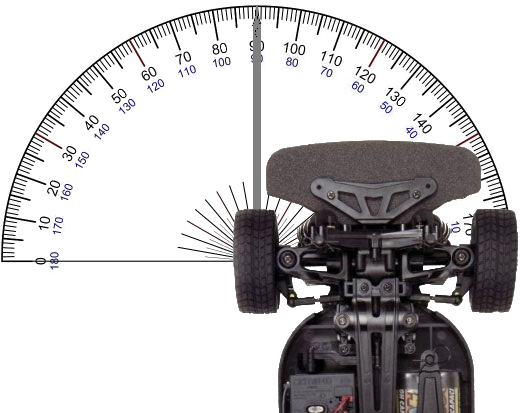
\includegraphics[width=5cm]{Bilder/u1Messung.png}
	\caption[Messng der Relation PWM-Stufe Servo zu Einschlagswinkel Räder]
		{Messng der Relation PWM-Stufe Servo zu Einschlagswinkel Räder (aus \cite{TT01} und \cite{Wim})}
	\label{pict:u1Mess}
\end{figure}

Als Ergebnis dieses Experimentes kam heraus, dass die Erhöhung um eine PWM-Stufe des Servomotors konstant eine Drehung der Räder um 0.0028 rad entspricht. In der Tabelle \ref{tab:physGR} aufgeführten Größen wurden hingegen direkt am oTToCAR gemessen, bzw. das Trägheitsmoment aus einem CAD-Modell \cite{TimMar} berechnet. 

\begin{table}[h!]
\centering
\begin{tabularx}{\columnwidth}{m{6cm}|m{4cm}|X}
  \textbf{Physikalische Größe} & \textbf{Exakter Wert}& \textbf{Einheit}\\\hline\hline 
	\rule{0pt}{1mm} & &\\
	Dichte der Luft & $\rho_{L}=1,204$ & $[\text{kg s}^{-1} ]$\\
	Erdbeschleunigung& $g=9,806$ & $[\text{m s}^{-2}]$\\
	Masse& $m=2,8$ & $[\text{kg}]$\\
  	Radabstand& $l=0,257$ & $[\text{m}]$\\
	Radius des Rades & $r=0,0335$ & $[\text{m}]$\\
	Übersetzungsfaktor Drehzahl Motor $\rightarrow$ Räder  & $\epsilon=5,52$ & $[\text{-}]$
\end{tabularx}
\caption{Direkt bestimmbare Parameter \label{tab:Pardir}}
\end{table} 

\subsection{Bestimmung von Parametern mithilfe von Schätzverfahren}
Die verbliebenen zu ermittelnden Parameter erfordern weit umfangreichere Messungen, wie zum Beispiel die Parameter für den Rollwiderstand und die Schräglaufübersetzung der Räder, die sich auch nicht direkt messen lassen. Für die Suche nach geeigneten Parametersätzen wird dabei ein Schätzverfahren benötigt, das anhand von anderen direkt messbaren Größen, die von den gesuchten Parametern abhängig sind, die zu bestimmenden Parameter indirekt ermitteln kann. 

\subsubsection{Positinsbestimmung mittels Kamera}
Die wohl charackteristischsten Messgrößen des Fahrzeuges sind seine Position und Geschwindigkeit. Anhand der gegebenen Zustandsgleichungen und aus logischen Überlegungen erkennt man eine starke Abhängigkeit zu allen gesuchten Parametern. Die Geschwindigkeitsmessung wird dabei intern vom Fahrzeug bereit gestellt. Sie wird ähnlich realisiert, wie die an einem Fahrrad. Durch auf den Rädern befestigte Neodymmagneten wird ein Magnetfeld aufgebaut, das durch Hall-Sensoren gemessen werden kann. Das Magnetfeld am Hall-Sensor ändert sich, sobald die Räder anfangen zu rotieren. Die Änderung des Magnetfeldes über die Zeit kann direkt in eine Geschwindigkeit umgerechnet werden. Eine Erhöhung der Anzahl von Magneten ermöglicht dabei eine beliebig hohe Auflösung der Geschwindigkeitsmessung. \\

(Bild)\\ 

Für die Positionsbestimmung wurde ein Testfeld gebaut und das Tracking mittels Kamera durchgeführt. Die technischen Anforderungen an das Tracking sind dabei ein ausreichend großes Testfeld, sowie eine geeignete Kamera zu wählen. Bei der Wahl der Kamera muss auf verschiedene Anforderungen Rücksicht genommen werden, die vor einem Beschaffung klar definiert werden müssen. In dem Fall eines sich schnell bewegenden Fahrzeuges ist die Bilderanzahl pro Sekunde sehr hoch zu gewichten, um Bewegungsunschärfe und fehlende Bewegungen zwischen zwei Bilder zu minimieren, welche die Messungen verfälschen können. Desweiteren spielt die Auflösung für Positionsgenauigkeit und die Schnittstellen der Kamera für hohe Datenraten ein große Rolle. 

(Skizze vom Aufbau)\\

Nach dem Aufbau des Parcours und der Installation der Kamera, muss die Kamera kalibriert werden. Die Kalibrierung ist notwendig, um die Symmetrien die durch den "`Fischaugeneffekt"' der Linse und der perspektivischen Verzerrung entstehen wieder herzustellen. Ein gängiges Verfahren zur Beseitigung der Linsenkrümmung und der perspektivischen Verzerrung ist die Kalibrierung mittels Schachbrettmuster. Die Beseitigung des Effektes der Linsenkrümmung wird mittels einer Vorwärtstransformation der Pixel des entkrümmten Bildes in das gekrümmte realisiert \cite{Zhang}. Der Algorithmus dahinter funktioniert folgerndermaßen:

\begin{enumerate}
	\item Generierung der Kamera-Matrix K, oder auch Matrix der intrinsischen Parameter mithilfer der "`Camera Calibration Toolbox for Matlab"' \citep{Calib}. Dabei charackterisieren die Einträge $f_x$, $f_y$ die Brennweite und $c_x$, $c_y$ bilden den Mittelpunkt der Linse  auf dem Kamerabild.
	\begin{align*}
	K = \begin{bmatrix}
	f_x &  0 & c_x\\ 
	0 & f_y & c_y\\ 
	0 & 0 & 1
	\end{bmatrix}
	\end{align*}  
	\item Normierung der verzerrten Pixelkoordinaten (Koordinate z' entfällt): 
	\setcounter{MaxMatrixCols}{20} 
	\begin{gather*}
	\begin{pmatrix} x'\\ y'\\ z' \end{pmatrix} = K^{-1} \cdot 
	\begin{bmatrix}
	n_{h,1} & n_{h,1} & ... & n_{h,1} & n_{h,1} & n_{h,2} & ... & n_{h,2} & ... & n_{h,i}\\
	n_{b,1} & n_{b,2} & ... & n_{b,j-1} & n_{b,j} & n_{b,1} & ... & n_{b,j} & ... & n_{b,j}\\
	1 & 1 & ... & 1 & 1 & 1 & ... & 1 & ... & 1\\
	\end{bmatrix} \\[1mm] \text{mit} \\[1mm]
	\begin{matrix}
	n_{h} = 1,2,3,..., \text{Höhe der Kameraauflösung}\\ 
	n_{b} = 1,2,3,..., \text{Breite der Kameraauflösung}
	\end{matrix}
	\end{gather*}
	\item Anwendung eines nichtlinearen Modells für die radiale Linsenkrümmung, um die verzerrten Koordinaten abzubilden. Dabei stammen die Parameter $k_1$,$k_2$ (Koeffizienten der radialen Verzerrung) und  $p_1$,$p_2$ (Koeffizienten der tangentialen Verzerrung) ebenfalls aus Schritt 1 und wurden mit \citep{Calib} berechnet.
	\begin{gather*}
	{x}'' = x'\cdot \left ( 1+k_1\cdot r + k_2\cdot r^2 \right )+2 p_1\cdot x'y'+p_2\cdot \left ( r+2{x}'^2 \right )\\
	{y}'' = y'\cdot \left ( 1+k_1\cdot r + k_2\cdot r^2 \right )+2 p_2\cdot x'y'+p_1\cdot \left ( r+2{y}'^2 \right )\\[1mm] \text{mit} \\[1mm]
	r=\sqrt{{x}'^2+{y}'^2}
	\end{gather*}
	\item Anschließend werden Projektionen erstellt, mithilfe dieser durch lineare Interpolation ein entzerrtes Bild erstellt werden kann. 
	\begin{align*}
	u = f_x \cdot {x}'' + c_x\\
	v = f_y \cdot {y}'' + c_y
	\end{align*}
\end{enumerate}

Anschließend wird die perspektivische Ansicht in eine orthogonale Draufsicht projeziert. Dafür müssen die Ecken eines Rechtecks, bzw. die Ecken des Parcours (falls alle Winkel rechteckig) auf dem Bild markiert und eine homographische Matrix gebildet werden, damit ein sogenannter "`Top View"' des Bildes erstellt werden kann. Diese Vorgehensweise ist bekannt unter dem Namen "`Inverse Perspective Mapping"' (\cite{Galway} und \cite{Peter}): 
\begin{enumerate}
	\item Generierung der extrinsischen Matrix $T_{ext}$ mithilfe von \citep{Calib}. Die Einträge stehen hierbei für die Translation in die entsprechende Richtung.
	\begin{align*}
	T = \begin{bmatrix}
	T_x \\ 
	T_y \\ 
	T_z 
	\end{bmatrix}
	\end{align*}  
	\item Ermittlung der Eckpunkte $P_1$, $P_2$, $P_3$ in Pixelkoordinaten und $P_4$ des Rechtecks/Parcours und der Seitenlängen in Pixeln oder Meter. 
	\begin{align*}
	P =& \begin{bmatrix}
	P_1 & P_2 & P_3 & P_4 \\
	1 & 1 & 1 & 1 	  
	\end{bmatrix} \text{\quad mit \quad} P_n = \binom{ x }{ y }\\[1mm]
	L =& \begin{bmatrix}
	0 & 0 & d\left(P_1 \rightarrow P_2 \right) & d\left(P_3 \rightarrow P_4 \right)\\
	0 & d\left(P_2 \rightarrow P_3 \right) & d\left(P_4 \rightarrow P_1 \right) & 0\\
	0 & 0 & 0 & 0 
	\end{bmatrix}	
	\end{align*}
	\item Rotation und Translation der Bildpunkte relativ zur Kameraposition mit anschließender Normierung und der Projektion in die Zielkoordinaten 
	\begin{align*}
	R =& \begin{bmatrix}
	\cos\left(\alpha \right) & -\sin\left(\alpha \right) & 0 \\
	\sin\left(\alpha \right) & \cos\left(\alpha \right) & 0 \\
	0 & 0 & 1 	  
	\end{bmatrix} \\[1mm]
	X_{rt} =& R \cdot L + T * \begin{bmatrix}
	1 & 1 & 1 & 1
	\end{bmatrix} \\[1mm]
	X_{Target} =& K \cdot X_{rt}^{-1} \cdot \begin{bmatrix}
 	X_{rt|3,1} & ... & X_{rt|3,4} \\ 
 	X_{rt|3,1} & ... & X_{rt|3,4} \\
 	X_{rt|3,1} & ... & X_{rt|3,4}
 	\end{bmatrix}	
	\end{align*}
	\item Mit der gewonnenen Projektion $X_{Target}$ lassen sich mit MATLAB unter der Verwendung von der Funktion \textit{homography2d} \cite{Peter}, \textit{maketform} und \textit{imtransform} \cite{Steve} das Bild im Anschluss perspektivisch entzerren.	
\end{enumerate}

(Workflow)    

(Bilder vom Parcours vor der Entzerrung und danach)

\subsubsection{Synchronisierung interner und externen Messdaten}
Nach der Aufnahme der externen und internen Messwerte, müssen diese für den ODE-Solver aufbereitet werden. Die Aufnahme der Messungen erfolg dabei durch ein mächtiges Framework names ROS (Robot Operating System), welches alle Messungen über einen Server koordiniert und den Zeitpunkte einer jeder Messung protokolliert. Da die externen Positionsdaten der Kamera einen Takt von 50 Hz und die internen der Geschwindigkeitsmessungen einen Takt von 100 Hz haben, sind diese nicht koexistent. Um diese Daten miteinander zu synchronisieren wurde die Methode der linearen Approximation gewählt, um zu jedem Zeitpunkt Messdaten vorrätig zu haben. Dies ermöglicht einen unkomplizierten Umgang der Daten in einem ODE-Solver. 

(Formel)

\subsubsection{Anwendung der Schätzverfahren}
Die zur Schätzung benötigten Messwerte ...Die Benutzung von Schätzverfahren erolgt mithilfe von zwei Optimierungsverfahren, inklusive einer für beide Verfahren einheitliche Kostenfunktion, zur redundanten Validierung eines gefundenen Satz von Parametern.  

\subsubsection{Ergebnisse}
In der Anwendung der Schätzverfahren revidierten sich einige der Annahmen aus \cite{VikAnd} und es mussten teilweise neue getroffen werden, um bessere Ergebnisse zu erreichen. Zum Beispiel wurde die Annahme getroffen, dass die Schräglaufübersetzung $C_{\alpha}$ von Vorder- und Hinterräder gleich ist. Jedoch ergaben sich bei einer Trennung der Schräglaufübersetzung von Vorder- und Hinterräder eindeutig bessere Ergebnisse. Zudem musste ein weiterer Parameter $\eta_M$ eingeführt werden, um den Wirkungsgrad des Drehmomentes zu beschreiben, welches vom Motor erzeugt auf die Räder geleitet wird. Somit ergaben sich folgende Parameter, die das Modell mit einer ausreichenden Genauigkeit beschreiben: 

\begin{table}[h!]
\centering
\begin{tabularx}{\columnwidth}{m{7cm}|m{4cm}|X}
  \textbf{Physikalische Größe} & \textbf{Exakter Wert}& \textbf{Einheit}\\\hline\hline 
	\rule{0pt}{1mm} & &\\
	Kraftverteilung Vorder- zu Hinterrad& $\gamma=0,5$ & $[\text{-}]$\\
	Reibungskoeffizient& $f_R=1,857$ & $[\text{-}]$\\
	Schräglaufübersetzung hinten& $C_{h,\alpha}=0,93$ & $[\text{-}]$\\
  	Schräglaufübersetzung vorn& $C_{v,\alpha}=1,1$ & $[\text{-}]$\\
  	Wirkungsgrad Drehmoment Motor $\rightarrow$ Räder& $\eta_M=0,55$ & $[\text{-}]$\\
	Zeitl. Verzögerung von $u_{1}$& $T_{V}=0,1$ & $[\text{s}]$
\end{tabularx}
\caption{Ergebnisse der geschätzten Parameter. \label{tab:ParSch}}
\end{table} 

(Bild Ergbnis Realität zu Simulation mit geschätzten Parametern, Aussage "`ausreichend"' definieren - sprich das Modell kann dem realen System für 2 Meter exakt auf ... Metern folgen, dass reicht aus um die MPC für einen Zeithorizont von ... Sekunden bei der Geschwindigkeit von ... M/s zu auszulegen. Da wir auch nicht mehr von der Wahrnehmung erhalten, ergibt sich eine korrekte Vorhersage)
